\chapter{Introdução}

	\section{Tema}
	
		O tema do trabalho é o desenvolvimento de um dispositivo que realize a medição da frequência respiratória dentro de uma faixa sensível para respostas psicofisiológicas. Este dispositivo deve possibilitar o monitoramento e a extração de dados que auxiliarão em estudos os quais correlacionam alguns parâmetros da frequência respiratória com funções psicofisiológicas, como aquelas observadas sob alterações cognitivas, emocionais, sob estresse  doenças mentais.
		
	\section{Delimitação}
		
		O objeto de estudo é um protótipo capaz de mensurar comportamentos respiratórios tais quais a frequência e o período de inspiração e expiração, para, a partir desse, analisar a viabilidade de desenvolvimento de um sistema com baixo custo voltado ao uso científico. As medições terão como finalidade a obtenção de dados, referentes à frequência respiratória, a serem utilizados em experimentos que vinculem comportamentos saudáveis e suas variantes clínicas à respiração humana. O estudo, limita-se à obtenção, processamento e exibição desses dados, não abrangendo, a priori, interpretações acerca das correlações obtidas em eventuais medições realizadas, além de possuir, em princípio, finalidade meramente científica, sem conter qualquer estudo sobre viabilidade comercial de produtos que venham a ser desenvolvidos.
		
	\section{Justificativa}
	
		Segundo Sebastião Gusmão \cite{gusmao2004historia}, a medicina como ciência, baseada na interpretação natural da doença e não em magia e empirismo, como ocorria na medicina arcaica, tem sua origem no século V a.C com Hipócrates (c. 460-375 a.C). Desde então, análises e estudos sobre o funcionamento do corpo humano, bem como as interações deste com o meio ambiente, vêm sendo realizados em constante evolução. Hoje, sabe-se que o organismo humano é composto de diversas partes que, em conjunto, garantem o seu funcionamento adequado. O corpo é, portanto, um sistema complexo no qual atuam diversas variáveis. Sendo assim, grande parte dos estudos científicos atuais voltam seus métodos e análises ao estudo dos parâmetros que possuem influências para o bom ou mal funcionamento do organismo. Atualmente, sabe-se que diversas doenças psicofisiológicas produzem variações no funcionamento normal do corpo, como alterações na produção de determinados hormônios, no batimento cardíaco, na pressão arterial ou na concentração de $CO_2$ no sangue. 
		
		Estudos recentes demonstram que é possível por exemplo, induzir pânico em ratos apenas alterando a concentração de $O_2$ ou de $CO_2$ do ar por eles respirado \cite{spiacci2015serotonin} \cite{spiacci2018panic}. A respiração humana é, assim como nos ratos, o processo natural responsável pela troca do $CO_2$ com o $O_2$.    
		
		Ao realizar uma análise de correspondência (correlação, regressão, inferência etc.) entre determinado comportamento biológico e algum quadro clínico específico, o 		pesquisador necessita realizar, de alguma maneira, a mensuração das variáveis que compõem o comportamento com acurácia e significado preditivo para a sensibilidade e a especificidade dos resultados. Nesse sentido, o desenvolvimento de um sistema de baixo custo capaz de coletar dados referentes ao comportamento respiratório torna-se parte essencial à evolução do estudo científico. 
		  
		Munido dessa motivação, neste trabalho, apresentam-se estudos para viabilidade do desenvolvimento de uma tecnologia com baixo custo capaz de monitorar o comportamento do fluxo respiratório de pacientes, servindo então como base para estudos científicos nas áreas de psicofisiologia e neurociência comportamental. 
		
	\section{Objetivos}
	
		O objetivo geral deste estudo é, então, construir um sistema (software e hardware) capaz de realizar a mensuração de dados referentes à frequência respiratória em humanos, incluindo parâmetros que possam ser utilizados em pesquisas psicofisiológicas. Desta forma, tem-se como objetivos específicos: (1) Realizar a mensuração da frequência respiratória (2) desenvolver os métodos de medida da frequência respiratória para extrair suas variantes no domínio do tempo e da frequência; e (3) Possibilitar a exportação dos dados para análises futuras.

	\section{Métodos}
	
		O sistema alvo deste trabalho foi projetado para ser constituído de duas partes:
		
		\begin{itemize}
			\item [1-] Software capaz de receber os dados de entrada, realizar operações matemáticas, exibir e exportar dados.
			\item [2-] Hardware capaz de realizar a aquisição do sinal respiratório, quantizar e se comunicar com o software.
		\end{itemize}
		
		O software é composto por um sistema capaz de realizar a leitura do hardware através de uma porta USB e por um sistema web programado em Python, utilizando o framework Flask, responsável por armazenar medições, bem como informações sobre pacientes e experimentos, em um banco de dados, realizar operações matemáticas, como análise de Fourier, e exibir os resultados em um gráfico interativo. 
		
		O hardware, por sua vez, foi projetado para ser o responsável pela aquisição da respiração, utilizando o termistor, que é um resistor variável à temperatura, escolhido principalmente por suas propriedades de autoaquecimento e pela variação exponencial de sua resistência em relação à mudança na temperatura, contrário a grande parte dos demais sensores que possuem uma relação linear entre essas variáveis. Trabalhar com um sensor de cuja curva característica é exponencial facilita detecções de pequenas variações na temperatura, gerando grandes mudanças na resistência, em contrapartida, adiciona complexidade ao sistema dado que trabalhar com relações lineares é, em geral, mais simples. A escolha do termistor é portanto perfeita porque sua contrapartida sequer implica em complicações para o sistema deste trabalho, dado que, em princípio, não interessa uma medição precisa da temperatura, mas sim o registro dos eventos de inspiração e expiração.
		
		Por derradeiro, o sistema completo, representado na figura \ref{fig:fluxo_sistema}, é composto de uma fonte capaz de entregar ao sensor corrente suficiente para que o termistor entre em estado de autoaquecimento e atinja uma temperatura alta o suficiente para se tornar sensível à variação provocada pelos fluxos de ar, um circuito de controle responsável por controlar a corrente de entrada no termistor, impedindo que esse queime ao aquecer indefinidamente, um microcontrolador que irá quantizar a leitura da tensão de entrada e enviar o sinal quantizado ao computador através de uma porta USB, um software responsável por realizar a leitura da porta USB e armazenar os dados em um arquivo .csv e um sistema web onde o pesquisador poderá acessar remotamente os resultados das medições, realizar operações matemática e análises gráficas.
				
		\begin{figure}[h!]
			\begin{center}
				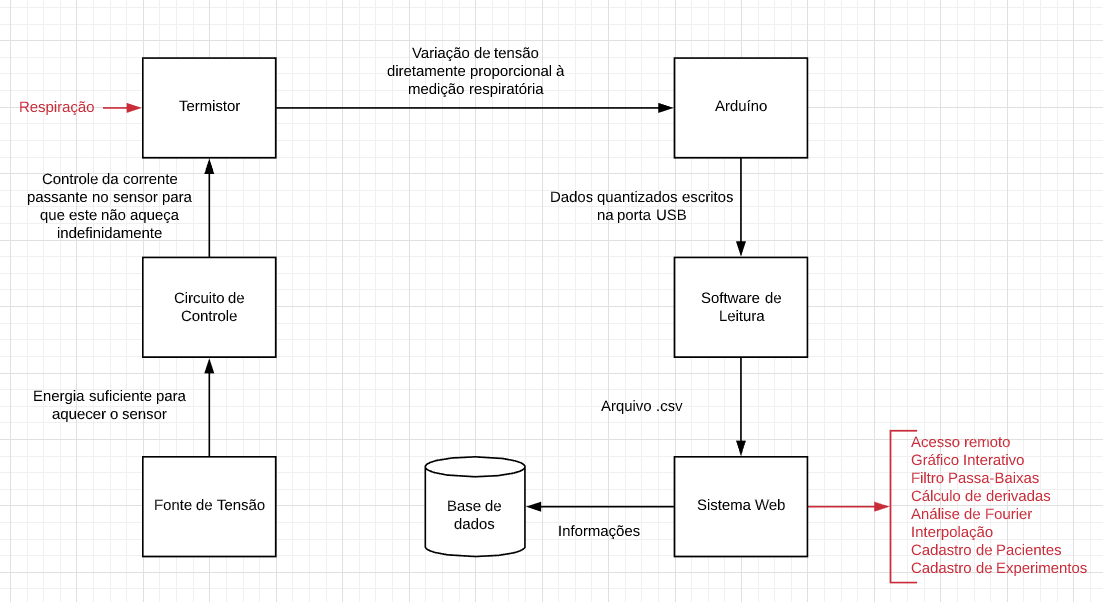
\includegraphics[width=1\linewidth]{images/fluxo_sistema.png}
				\caption{Representação completa do sistema}
				\label{fig:fluxo_sistema}
			\end{center}
		\end{figure}
		
	
	\section{Organização do Trabalho}
	
		Nos próximos capítulos serão apresentados em mais detalhes as aplicações, o desenvolvimento e os resultados obtidos com esse trabalho, organizados da seguinte forma:
		
		O capítulo 2 apresentará a motivação para o desenvolvimento do sistema, as aplicações no campo da medicina e um resumo do funcionamento fisiológico da respiração humana. 
		
		O capítulo 3 tratará sobre desenvolvimento do sistema, hardware e software bem como o raciocínio por trás da arquitetura.
		
		O capítulo 4 será destinado à conclusão desse projeto, com o protótipo construído no último ciclo de desenvolvimento, limitações encontradas ao longo das etapas e também possíveis melhorias para trabalhos futuros.
